\documentclass[twoside]{report}
\usepackage[italian]{babel}
\usepackage[utf8]{inputenc}
\usepackage{amsmath}
\usepackage{amsthm}
\usepackage{amsfonts}
\usepackage{amssymb}
\usepackage{cancel}
\usepackage[margin=1in]{geometry}
\usepackage{hyperref}
\usepackage{graphicx}
\usepackage{wrapfig}
\usepackage{listings}
\usepackage{algorithm}
\usepackage[noend]{algpseudocode}
\usepackage{fancyhdr}

\graphicspath{{./images/}}

\makeatletter
\renewenvironment{abstract}{%
    \if@twocolumn
        \section*{\abstractname}%
    \else
        \begin{center}%
            {\bfseries \abstractname\vspace{-.5em}\vspace{\z@}}%
        \end{center}%
        \small
        \begin{quotation}
    \fi}
    {\if@twocolumn\else\end{quotation}\fi}
\makeatother

% Definizione di nuovi comandi per definizioni, caso base e passo induttivo
\theoremstyle{definition}
\newtheorem{definition}{Definizione}[chapter]
\newtheorem*{basecase}{Caso Base}
\newtheorem*{inductivecase}{Passo Induttivo}

% Definizione per il package algorithm
% Definizioni di int, boolean, float
\algnewcommand\Int{\textbf{int}\ }
\algnewcommand\Bool{\textbf{boolean}\ }
\algnewcommand\Float{\textbf{float}\ }
\algnewcommand\To{\textbf{to}\ }
\algnewcommand\DownTo{\textbf{downto}\ }
% Definizione di header e footer

% Definizione dei teoremi
\newtheorem{theorem}{Teorema}[chapter]

\title{Appunti di Algoritmi e Strutture Dati}
\author{Luca Facchini (mat. 245965)}
\date{A.A. 2024/2025}



\fancypagestyle{chapterInit}{
    \fancyhf{}
    \renewcommand{\headrulewidth}{0pt}
    \fancyhead{}
    \fancyfoot{}
    \fancyfoot[LE,RO]{\thepage}
    \fancyfoot[LO,RE]{"Appunti di Algoritmi e Strutture Dati" di Luca Facchini}
}
\fancypagestyle{stdPage}{
    \fancyhead{}
    \fancyhead[RO,LE]{\leftmark}
    \fancyhead[RE,LO]{\rightmark}
    \fancyfoot{}
    \fancyfoot[LE,RO]{\thepage}
    \fancyfoot[LO,RE]{"Appunti di Algoritmi e Strutture Dati" di Luca Facchini}
}

\begin{document}
    \begin{titlepage}
        \centering  % Center everything on the title page
        {\Huge\textbf{Appunti di Algoritmi e Strutture Dati}} \\[1cm] % Title
        \vspace{0.5cm}
        
        {\Large Luca Facchini} \\ % Author name
        \vspace{0.3cm}
        {\large Matricola: 245965} \\[2cm] % Additional author info
        
        {\large Corso tenuto dal prof. Montresor Alberto} \\[0.3cm] % Course information
        {\large Università degli Studi di Trento} \\[1.5cm]
        
        {\large A.A. 2024/2025} \\[3cm] % Academic year
        
        % Abstract section with spacing control
        \vfill
        \begin{abstract}
            Appunti del corso di Algoritmi e Strutture Dati tenuto dal prof. Montresor Alberto presso l'Università degli Studi di Trento nell'anno accademico 2024/2025.
        \end{abstract}
        
        \vfill  % Pushes the content to the center vertically
    \end{titlepage}
    \pagestyle{stdPage}
    \renewcommand{\headheight}{14.5pt}
    \begingroup
        \tableofcontents
        \thispagestyle{stdPage}
    \endgroup
    
    \chapter{Analisi di Algoritmi}
\thispagestyle{chapterInit}
\section{Modelli di calcolo}
    \subsection{Definizioni}    
        \subsubsection{Complessità}
            \begin{definition}
                La \textbf{complessità} di un algoritmo è definita come la quantità di \textbf{tempo} necessaria per eseguirlo in funzione della \textbf{dimensione dell'input}.
            \end{definition}
            Le domande spontanee che ci si pone sono dunque:
            \begin{itemize}
                \item Come definire la dimensione dell'input?
                \item Come misurare il tempo?
            \end{itemize}
        \subsubsection{Dimensione dell'input}
            \begin{definition}
                Per definire la \textbf{dimensione dell'input} abbiamo due criteri:
                \begin{description}
                    \item[Costo Logaritmico] Il costo logaritmico è definito come il numero di bit necessari per rappresentare l'input.
                    \item[Costo Uniforme] La taglia dell'input è definita come il numero di elementi da cui è composto. 
                \end{description}
            \end{definition}
            Ma in molti casi possiamo assumere che tutti gli elementi siano rappresentati dallo stesso numero di bit costante e che coincidono a meno di costante moltiplicativa
        \subsubsection{Tempo}
            \begin{definition} 
                Un'istruzione si considera elementare se può essere eseguita in tempo "costante" dal processore, dunque un esempio ne è la moltiplicazione o una funzione matematica ad esempio $\cos(d)$, ma una istruzione come il massimo tra due numeri non è elementare.
            \end{definition}
        \subsubsection{Modello di calcolo}
            \begin{definition}
                Un modello di calcolo è definito come la rappresentazione astratta di un calcolatore che rispetta i seguenti criteri:
                \begin{description}
                    \item[Astrazione] Il modello deve permettere di nascondere i dettagli.
                    \item[Realismo] Il modello deve riflettere una situazione reale.
                    \item[Potenza Matematica] Il modello deve permettere di dimostrare "formalmente" la complessità di un algoritmo.    
                \end{description}
            \end{definition}
            Esempio di modello di calcolo è la \textbf{Macchina di Turing}.
    \subsection{Esempi di Analisi}
        \subsubsection{Tempo di calcolo $\min()$}
            Sappiamo che ogni istruzione richiede un tempo costante per essere eseguita e che ogni operazione potenzialmente ha una costante diversa dalle altre e che ogni istruzione viene eseguita un numero di volte diversa dalle altre.
            
            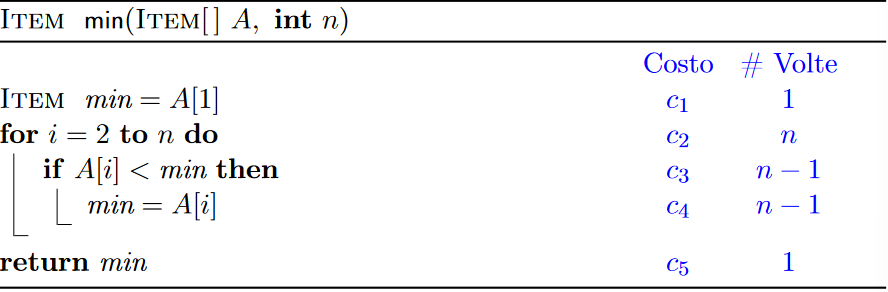
\includegraphics[width=0.9\textwidth]{01/calcoloMin.png}
            
            Otteniamo quindi che il tempo di calcolo è:
            \[
                \begin{aligned}
                    T(n)=&c_1+c_2n+c_3(n-1)+c_4(n-1)+c_5\\
                    =&(c_2+c_3+c_4)n+(c_1+c_5-c_3-c_4) = an+b
                \end{aligned}
            \]
        \subsubsection{Tempo di calcolo di $\operatorname{binarySearch}()$}
            In questo algoritmo il vettore viene suddiviso in due parti:
            $ \text{Parte SX: } \left\lfloor(n-1)/2\right\rfloor $ e $ \text{Parte DX: } \left\lfloor n/2\right\rfloor $.
            
            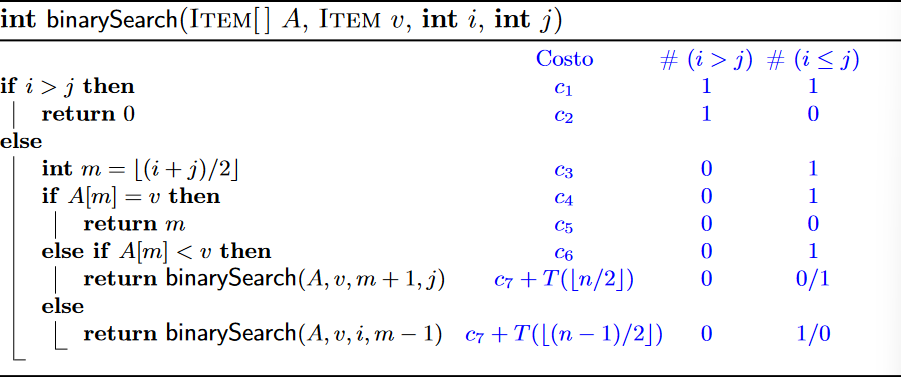
\includegraphics[width=0.9\textwidth]{01/calcoloBinarySearch.png}
            
            A questo punto dobbiamo fare delle assunzioni:
            \begin{itemize}
                \item Assumiamo che la $ n $ potenza di $ 2 $ sia: $ n = 2^k $.
                \item L'elemento cercato non è presente.
                \item Ad ogni passo andiamo sempre a destra in quanto il numero di elementi da valutare è maggiore: $ n/2 $.
            \end{itemize}
            possiamo ora suddividere il problema in due casistiche:
            $$
                \begin{aligned}
                    i>j\quad & (n=0) & T(n)=&c_1 + c_2\\
                    i\leq j\quad & (n>0) & T(n)=&T(n/2) + c_1 + c_2 + c_3 + c_4 + c_6 + c_7\\
                        &&=&T(n/2) + d
                \end{aligned}
            $$
            unendo i due casi otteniamo la \textbf{Relazione di ricorrenza}:
            $$
                T(n)=
                    \begin{cases}
                        c& \text{se } n=0\\
                        T(n/2) +d & \text{se } n>0
                    \end{cases}
            $$
            ottenuta la relazione generalmente per un numero $ n $ di elementi otteniamo che il tempo è dato da:
            $$
                \begin{aligned}
                    T(n)=&T(n/2)+d&\\
                    =&T(n/4)+2d&\\
                    &\hdots\\
                    =&T(1)+kd&\\
                    =&T(0)+(k+1)d&\\
                    =&kd+(c+d) &= d\log n + e
                \end{aligned}
            $$
            ottenendo quindi che il tempo di calcolo è $ O(\log n) $ di natura logaritmica.
    \subsection{Ordini di Complessità}
        \begin{table}[h]
            \centering
            \begin{tabular}{|c|c|c|c|c|c|}
                \hline
                $ f(n) $ & $ n=10^1 $ & $ n=10^2 $ & $n=10^3 $ & $n=10^4 $ & \textbf{Tipo} \\
                \hline
                $ \log n $ & 3 & 6 & 9 & 13 & Logaritmica \\
                \hline
                $ \sqrt{n} $ & 3 & 10 & 31 & 100 & sub-lineare \\
                \hline
                $ n $ & 10 & 100 & 1000 & 10000 & Lineare \\
                \hline
                $ n\log n $ & 30 & 664 & 9965 & 132877 & log-lineare \\
                \hline
                $ n^2 $ & $10^2$ & $10^4$ & $10^6$ & $10^8$ & Quadratica \\
                \hline
                $ n^3 $ & $10^3$ & $10^6$ & $10^9$ & $10^{12}$ & Cubica \\
                \hline
                $ 2^n $ & $1024$ & $10^{30}$ & $10^{301}$ & $10^{3010}$ & Esponenziale\\
                \hline
            \end{tabular}
        \end{table}
\section{Notazione asintotica}
\label{sec:notazioneAsintotica}
    \subsection{Notazioni \texorpdfstring{$ O $, $ \Omega $, $ \Theta $}{O, Omega, Theta}}
        \subsubsection{Notazione $ O $}
            \begin{definition}
                Sia $ g(n) $ una funzione di costo; indichiamo con $ O(g(n)) $ l'insieme delle funzioni $ f(n) $ tali per cui: 
                $$ \exists c>0,\ \exists m\geq 0: f(n) \leq cg(n),\ \forall n\geq m $$
            \end{definition}
            La seguente notazione si legge: $ f(n) $ è "O grande" (big O) di $ g(n) $, con un abuso di notazione si scrive $ f(n)=O(g(n)) $\footnote{\label{fn:note1} Questo è un abuso di notazione in quanto $ O(g(n)) $ è una classe di funzioni e non può essere eguagliata una singola funzione, il simbolo più appropriato sarebbe $ f(n)\in O(g(n)) $}
            . Inoltre per la precedente definizione possiamo dire che $ g(n) $ è un \textbf{limite asintotico superiore} per $ f(n) $, in quanto dopo qualche valore $ m $ la funzione $ g(n) $ è sempre maggiore di $ f(n) $. Inoltre per questo motivo sappiamo che $ f(n) $ cresce al più come $ g(n) $.
        \subsubsection{Notazione $ \Omega $}
            \begin{definition}
                Sia $ g(n) $ una funzione di costo; indichiamo con $ \Omega(g(n)) $ l'insieme delle funzioni $ f(n) $ tali per cui: 
                $$ \exists c>0,\ \exists m\geq 0: f(n) \geq cg(n),\ \forall n\geq m $$
            \end{definition}
            La seguente notazione si legge: $ f(n) $ è "Omega" di $ g(n) $, con un abuso di notazione si scrive $ f(n)=\Omega(g(n)) $\footref{fn:note1}. Inoltre per la precedente definizione possiamo dire che $ g(n) $ è un \textbf{limite asintotico inferiore} per $ f(n) $, in quanto dopo qualche valore $ m $ la funzione $ g(n) $ è sempre minore di $ f(n) $. Inoltre per questo motivo sappiamo che $ f(n) $ cresce almeno come $ g(n) $.
        \subsubsection{Notazione $ \Theta $}
            \begin{definition}
                Sia $ g(n) $ una funzione di costo; indichiamo con $ \Theta(g(n)) $ l'insieme delle funzioni $ f(n) $ tali per cui: 
                $$ \exists c_1>0,\ \exists c_2>0,\ \exists m\geq 0: c_1g(n) \leq f(n) \leq c_2g(n),\ \forall n\geq m $$
            \end{definition}
            La seguente notazione si legge: $ f(n) $ è "Theta" di $ g(n) $, con un abuso di notazione si scrive $ f(n)=\Theta(g(n)) $\footref{fn:note1}. Inoltre per la precedente definizione possiamo dire che $ f(n) $ cresce esattamente come $ g(n) $, detto ciò $ f(n)= \Theta(g(n)) $ se e solo se $ f(n)=O(g(n)) $ e $ f(n)=\Omega(g(n)) $.
        \subsubsection*{Esempio grafico}
            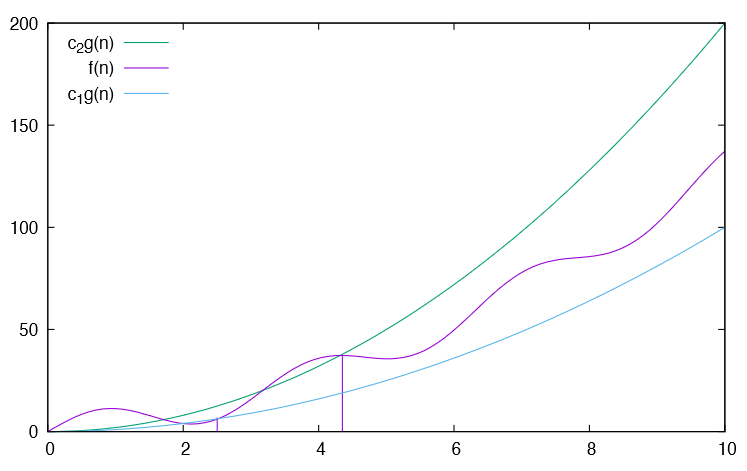
\includegraphics[width=0.5\textwidth]{01/graficoNotazioni.png}
    \subsection{Esempi e Esercizi}
        \subsubsection{Esempio 1}
            $$
                f(n) = 10n^3 + 2n^2 + 7 \stackrel{?}{=} O(n^3)
            $$
            Dobbiamo provare che $ \exists c>0,\ \exists m\geq 0: f(n) \leq cn^3,\ \forall n\geq m $.
            $$
                \begin{aligned}
                    f(n) =& 10n^3 + 2n^2 + 7\\
                    \leq & 10n^3 + 2n^3 + 7 &\quad \forall n \geq 1\\ 
                    \leq & 10n^3 + 2n^3 + n^3 &\quad  \forall n \geq \sqrt[3]{7}\\
                    = & 13 n^3 \stackrel{?}{\leq} cn^3
                \end{aligned}
            $$
            Che è verificata per qualsiasi $ c \geq 13 $ e $ m \geq \sqrt[3]{7} $, arrotondiamo $m$ ad un intero superiore ottenendo $ m = 2 $. 
            
            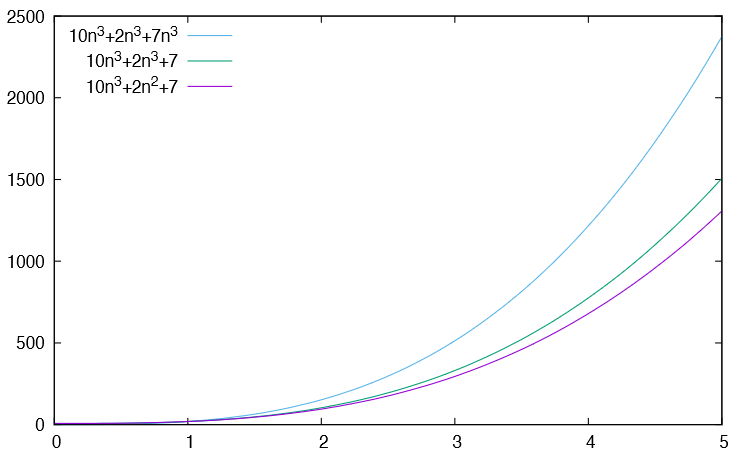
\includegraphics[width=0.5\textwidth]{01/graficoEs1.png}
\section{Complessità problemi v/s algoritmi}
    \subsection{Moltiplicazione numeri complessi}
        Per moltiplicare numeri complessi bisogna svolgere la seguente operazione:
        $$
            (a+bi)(c+di) = [ac-bd]+[ad+bc]i
        $$
        dunque dai parametri $ a,b,c,d $ otteniamo che il risultato da restituire: $ ac-bd $ e $ ad+bc $.
        \paragraph{Domande}
            Considerando che addizioni e sottrazioni costino $ c_1 = 0.01 $ e moltiplicazione costi $ c_2 = 1 $ possiamo chiederci:
            \begin{itemize}
                \item Quanto costa l'algoritmo?
                \item Si può fare meglio?
                \item Qual'è il ruolo del modello di calcolo?
            \end{itemize}
            Dato che si devono fare almeno 4 moltiplicazioni e 2 somme otteniamo che il costo totale è $ 4c_2 + 2c_1 = 4.02 $.
            
            Ora si può fare meglio? La risposta è no in quanto se si potesse fare meglio si potrebbe fare meglio allora bisognerebbe trovare un algoritmo che esegua meno di 4 moltiplicazioni e 2 somme, ma per fare ciò bisognerebbe cambiare il modello di calcolo.
    \subsection{Sommare numeri binari}
        \subsubsection{Algoritmo elementare della somma - $ \operatorname{sum}() $}
            Ipotizziamo che l'operazione da fare sia la somma di due bit singoli e generare il riporto, assegniamo a questa operazione costo $ c $.
            Dopo ciò indichiamo con $ n $ il numero massimo di bit tra i due numeri da sommare, otteniamo dunque che:
            \begin{itemize}
                \item Richiede di esaminare tutti gli $ n $ bit
                \item Costo totale $ cn = O(n) $
            \end{itemize}
        \subsubsection{Esiste allora un algoritmo più efficiente?}
            La risposta è no in quanto se esistesse un algoritmo di tale genere allora potremmo cambiare un solo bit di uno dei due numeri e ottenere un risultato diverso senza che l'algoritmo lo vada ad analizzare, il che è impossibile.
    \subsection{Moltiplicare numeri binari}
        \subsubsection{Algoritmo elementare del prodotto - $\operatorname{prod}()$}
            L'operazione elementare per moltiplicare due numeri binari è la seguente:
            $$
                \begin{array}{c c c c c c c c c c c c c c c}
                    & & & & & & & 1 & 0 & 1 & 1 & 1 & 0 & 1 & *\\
                    & & & & & & & 1 & 1 & 0 & 1 & 1 & 1 & 0 & \\
                    \hline
                    & & & & & & & 0 & 0 & 0 & 0 & 0 & 0 & 0 &\\
                    & & & & & & 1 & 0 & 1 & 1 & 1 & 0 & 1 & &\\
                    & & & & & 1 & 0 & 1 & 1 & 1 & 0 & 1 & & &\\
                    & & & & 1 & 0 & 1 & 1 & 1 & 0 & 1 & & & &\\
                    & & & 0 & 0 & 0 & 0 & 0 & 0 & 0 & & & & &\\
                    & & 1 & 0 & 1 & 1 & 1 & 0 & 1 & & & & & &\\
                    & 1 & 0 & 1 & 1 & 1 & 0 & 1 & & & & & & &\\
                    \hline
                    1 & 0 & 0 & 1 & 1 & 1 & 1 & 1 & 1 & 1 & 0 & 1 & 1 & 0\\
                \end{array}
            $$
            deduciamo che:
            \begin{itemize}
                \item Dobbiamo accedere a tutti i bit
                \item Il costo totale è $ cn^2 = O(n^2) $ perché dobbiamo fare $ n $ somme di $ n $ bit.
            \end{itemize}
        \subsubsection{Soluzione Divide-et-impera}
            La base del principio \textbf{Divide-et-impera} è la seguente:
            \begin{description}
                \item[Divide] Dividere il problema in sotto-problemi più piccoli.
                \item[Impera] risolvi i sotto-problemi in modo ricorsivo.
                \item[Combina] combina le soluzioni dei sotto-problemi per ottenere la soluzione del problema originale.  
            \end{description}
            La soluzione divide-et-impera per il problema della moltiplicazione binaria è la seguente:
            $$
                \begin{aligned}
                    \begin{aligned}
                        X=& a\cdot 2^{n/2} + b\\
                        Y=& c\cdot 2^{n/2} + d\\
                        XY =& ac\cdot 2^n + (ad+bc)\cdot 2^{n/2} + bd
                    \end{aligned}
                    &\quad
                    \begin{aligned}
                        X &= \stackrel{a}{\text{Parte SX}}\quad \stackrel{b}{\text{Parte DX}}\\
                        Y &= \stackrel{c}{\text{Parte SX}}\quad \stackrel{d}{\text{Parte DX}}
                    \end{aligned}
                \end{aligned}
            $$
            Ora possiamo scrivere l'algoritmo:
            \begin{algorithm}
                \caption{boolean[ ] pdi(boolean[ ] X, boolean[ ] Y, int n)}\label{alg:pdi}
                \begin{algorithmic}[1]
                    \If{$n=1$}
                        \State \Return $X[1]\cdot Y[1]$
                    \Else
                        \State spezza $X$ in $a$ e $b$ e $Y$ in $c$ e $d$
                        \State \Return pdi($a,c,n/2$)$\cdot 2^n$ + (pdi($a,d,n/2$) + pdi($b,c,n/2$))$\cdot 2^{n/2}$ + pdi($b,d,n/2$)
                    \EndIf
                \end{algorithmic}
            \end{algorithm}
            La funzione di costo associata all'algoritmo è:
            $$
                T(n)=\begin{cases}
                    c_1 & n=1\\
                    4T(n/2)+c_2\cdot n &  n>1
                \end{cases}
            $$
            \textbf{Nota:} moltiplicare per $2^n$ corrisponde a uno shift a sinistra di $n$ posizioni, svolta in tempo lineare.

            Ora in quanto abbiamo $ 4 $ chiamate ricorsive, assumendo che $c_1$ sia il tempo per moltiplicare due bit e che $ c_2 $ sia il tempo per sommare due numeri binari otteniamo che il tempo di calcolo è $ c_2 \cdot 4^i \cdot \frac{n}{2^i} = T(1) \cdot 4^{\log_2 n} = c_1 \cdot n^{\log_2 4} = c_1 \cdot n^2 $.
            \subparagraph{Ma allora è possibile fare meglio?}
            Long story short: si in quanto è stato provato nel 2021 l'esistenza di un algoritmo di complessità $ O(n\log n) $. 
\section{Algoritmi di Ordinamento}
    \paragraph{Introduzione} L'obbiettivo di questa sezione è valutare la complessità degli algoritmi in base all'input, in alcuni casi gli algoritmi si comportano differentemente in base all'input se siamo a conoscenza dell'input questa ci consente di scegliere un algoritmo più adeguato alla nostra soluzione.
    \paragraph{Come analiziamo gli algoritmi}
        Possiamo analizzare l'efficienza degli algoritmi in base a diversi casi:
        \subparagraph{Caso Pessimo}
            Questa analisi è la più importante in quanto sappiamo che questa restituisce il limite superiore al tempo di esecuzione qualsiasi sia l'input.
        \subparagraph{Caso Medio}
            Questa analisi è la più complessa in quanto bisogna definire il "caso medio" e cosa si intende per "medio", ma è utile con una distribuzione uniforme degli input.
        \subparagraph{Caso Ottimo}
            Utile solo se conosciamo qualcosa sull'input, altrimenti non risulta utile se abbiamo un input arbitrario.
    \subsection{Selection Sort}
        Algoritmo Selection Sort:
        \begin{algorithm}
            \caption{selectionSort(Item[ ] A, \Int n)}\label{alg:selectionSort}
            \begin{algorithmic}[1]
                \For{$i=1$ \To $n-1$}
                    \State \Int $min \gets \operatorname{min}(A,i,n)$
                    \State $A[i]$ $\leftrightarrow$ $\operatorname{min}(A,i,n) $
                \EndFor
            \end{algorithmic}
        \end{algorithm}

        Algoritmo di supporto min:
        \begin{algorithm}
            \caption{int min(Item[ ] A, \Int i, \Int n)}\label{alg:min}
            \begin{algorithmic}[1]
                \State \Int min $\gets i$
                \For{$j=i+1$ \To $n$}
                    \If{$A[j]<A[min]$}
                        \State min $\gets j$
                    \EndIf
                \EndFor
                \State \Return min
            \end{algorithmic}
        \end{algorithm}
        Avendo analizzato il seguente algoritmo notiamo come in ogni caso, ottimo, medio e pessimo, il "ciclo" esterno della funzione $ \operatorname{selectionSort}() $ viene eseguito $ n-1 $ volte, mentre il ciclo interno della funzione $ \operatorname{min}() $ viene eseguito $ n-i $ dove $ i $ è il valore dell'iterazione del ciclo esterno, quindi $ n-1 + n-2 + n-3 + \ldots + 1 = \frac{n(n-1)}{2} $ volte, otteniamo quindi che il tempo di calcolo è $ O(n^2) $ in quanto questo si può approssimare a $ \frac{n^2}{2} $.
        $$  
            \sum_{i=1}^{n-1} n-i = \sum_{i=1}^{n-1} i = \frac{n(n-1)}{2}= O(n^2)
        $$
    \subsection{Insertion Sort}
        L'algoritmo di insertion sort è efficiente per ordinare piccoli insiemi, il concetto dietro a questo si bassa sull'inserimento dell'elemento preso in analisi al posto giusto.
        
        Algoritmo Insertion Sort:
        \begin{algorithm}
            \caption{insertionSort(Item[ ] A, \Int n)}\label{alg:insertionSort}
            \begin{algorithmic}[1]
                \For{$i=2$ \To $n$}
                    \State Item $temp \gets A[i]$
                    \State \Int $j \gets i$
                    \While{$j>1$ and $A[j-1]>temp$}
                        \State $A[j] \gets A[j-1]$
                        \State $j \gets j-1$
                    \EndWhile
                    \State $A[j] \gets temp$
                \EndFor
            \end{algorithmic}
        \end{algorithm}
        
        Il costo di esecuzione non dipende esclusivamente dalla dimensione ma anche dall'ordine degli elementi in ingresso.
        \subparagraph{Caso Pessimo} Il costo dunque nel \textbf{caso pessimo} è $ O(n^2) $ in quanto vengono eseguiti $ n-1 $ cicli esterni e $ n-1 $ cicli interni, ottenendo dunque $ (n-1) + (n-2) + \ldots + 1 = \frac{n(n-1)}{2} = O(n^2) $.
        \subparagraph{Caso Medio }Nel \textbf{caso medio} il costo rimane $ O(n^2) $ in quanto il ciclo interni viene eseguito $ n/2 $ volte, ottenendo dunque $ \frac{n(n-1)}{4} = O(n^2) $.
        \subparagraph{Caso Ottimo} Nel \textbf{caso ottimo} il costo è $ O(n) $ in quanto il ciclo interno non viene mai eseguito.
        
        Questo ci porta a dire che il $ \operatorname{insertionSort}() $ è un algoritmo di ordinamento utile nei casi in cui l'input è già ordinato o quasi ordinato, nei casi nei quali non conosciamo la natura dell'input è meglio utilizzare un algoritmo di ordinamento differente.
    \subsection{Merge Sort}
        L'algoritmo di $ \operatorname{mergeSort}() $ è un algoritmo di ordinamento basato sul principio \textbf{divide-et-impera}.
        \begin{description}
            \item[Divide:] Spezza virtualmente il vettore di $ n $ elementi in sotto-vettori di $ n/2 $ elementi.
            \item[Impera:] Chiama $ \operatorname{mergeSort}() $ ricorsivamente sui due sotto-vettori.
            \item[Combina:] Unisci (\textbf{merge}) i due sotto-vettori ordinati in un unico vettore ordinato. 
        \end{description}
        In input si ha:
        \begin{itemize}
            \item $ A $: vettore di $ n $ elementi.
            \item $ \text{start}, \text{end}, \text{mid} $ sono tali che $ 1\leq \text{start} < \text{mid} < \text{end} \leq n $.
            \item I sotto-vettori $ A[\text{start},\ldots,\text{mid}] $ e $ A[\text{mid}+1,\ldots,\text{end}] $ sono ordinati.
        \end{itemize}
        In output si hanno i due sotto-vettori fusi in un unico sotto-vettore ordinato, tramite un vettore di appoggio $ B $.

        Funzione di appoggio $\operatorname{Merge}$:
        \begin{algorithm}
            \caption{Merge(Item[ ] A, \Int start, \Int end, \Int mid)}\label{alg:merge}
            \begin{algorithmic}[1]
                \State \Int $i,j,k,h$
                \State \Int $i \gets \text{start}$
                \State \Int $j \gets \text{mid}+1$
                \State \Int $k \gets \text{start}$
                \While {$i \leq \text{mid}$ and $j \leq \text{end}$}
                    \If{$A[i] \leq A[j]$}
                        \State $B[k] \gets A[i]$
                        \State $i \gets i+1$
                    \Else
                        \State $B[k] \gets A[j]$
                        \State $j \gets j+1$
                    \EndIf
                    \State $k \gets k+1$
                \EndWhile
                \State $j \gets \text{end}$
                \For {$h=\text{mid}$ \DownTo $i$}
                    \State $A[j] \gets A[h]$
                    \State $j \gets j-1$
                \EndFor
                \For {$j=\text{start}$ \To $k-1$}
                    \State $A[j] \gets B[j]$
                \EndFor
            \end{algorithmic}
        \end{algorithm}
        
        Il costo computazionale di $ \operatorname{Merge}() $ è $ O(n) $, questa è la base del costo computazionale di $ \operatorname{mergeSort}() $.
        \newpage % Usato per evitare che l'algoritmo venga spezzato tra due pagine diverse
        Funzione completa $ \operatorname{mergeSort}() $:

        \begin{algorithm}
            \caption{mergeSort(Item[ ] A, \Int start, \Int end)}\label{alg:mergeSort}
            \begin{algorithmic}[1]
                \If{$\text{start}<\text{end}$}
                    \State \Int $mid \gets (\text{start}+\text{end})/2$
                    \State mergeSort($A,\text{start},\text{mid}$)
                    \State mergeSort($A,\text{mid}+1,\text{end}$)
                    \State merge($A,\text{start},\text{end},\text{mid}$)
                \EndIf
            \end{algorithmic}
        \end{algorithm}

        Assumendo per semplificare che $ n = 2^k $ dove $ k $ è un intero allora l'altezza dell'albero è esattamente $ k = \log n $, in questo modo tutti i sotto-vettori hanno dimensione che è potenza di 2.
        Così facendo il costo computazionale di $ \operatorname{mergeSort}() $ è:
        $$
            T(n)=\begin{cases}
                c & n=1\\
                2T(n/2)+dn & n>1
            \end{cases}
        $$
        dove $ c $ è il costo di un'operazione elementare, $ d $ è il costo di $ \operatorname{Merge}() $ e $ n $ è il costo di copiare i valori da $ B $ a $ A $.
    \chapter{Analisi di funzioni}
\thispagestyle{chapterInit}
\section{Notazione asintotica}
    \subsection{Definizioni}
        Si rimanda al \hyperref[sec:notazioneAsintotica]{sezione 1.2} per le definizioni di $O$, $\Omega$ e $\Theta$.
\section{Proprietà della notazione asintotica}
    \subsection{Regola Generale}
        Da qui si prende in considerazione la seguente espressione polinomiale:
        $$
            f(n) = a_kn^k + a_{k-1}n^{k-1} + \ldots + a_1n + a_0, \quad a_k > 0 \Rightarrow f(n) = \Theta(n^k)
        $$
        \paragraph{Limite Superiore} $ \exists c>0, \exists m\geq 0: f(n)\leq cn^k,\forall n\geq m $
            $$
                \begin{aligned}
                    f(n)=&a_kn^k + a_{k-1}n^{k-1} + \ldots + a_1n + a_0 \\
                    \leq& a_kn^k + \left|a_{k-1}\right|n^{k-1} + \ldots + \left|a_1\right|n + \left|a_0\right| \\
                    \leq& a_kn^k + \left|a_{k-1}\right|n^k + \ldots + \left|a_1\right|n^k + \left|a_0\right|n^k \\
                    =& (a_k + \left|a_{k-1}\right| + \ldots + \left|a_1\right| + \left|a_0\right|)n^k \quad& \forall n\geq 1\\
                    \stackrel{?}{\leq}& cn^k
                \end{aligned}
            $$
            questa è vera per $ c\geq \left(a_k + \left|a_{k-1}\right| + \ldots + \left|a_1\right| + \left|a_0\right| \right) >0$ e per $m=1$
        \paragraph{Limite Inferiore} $ \exists d > 0, \exists m\geq 0: f(n)\geq dn^k,\forall n\geq m $
            $$
                \begin{aligned}
                    f(n)=&a_kn^k + a_{k-1}n^{k-1} + \ldots + a_1n + a_0 \\
                    \geq& a_kn^k - \left|a_{k-1}\right|n^{k-1} - \ldots - \left|a_1\right|n - \left|a_0\right| \\
                    \geq& a_kn^k - \left|a_{k-1}\right|n^k - \ldots - \left|a_1\right|n^k - \left|a_0\right|n^k \\
                    =& (a_k - \left|a_{k-1}\right| - \ldots - \left|a_1\right| - \left|a_0\right|)n^k \quad& \forall n\geq 1\\
                    \stackrel{?}{\geq}& dn^k
                \end{aligned}
            $$
            questa è vera se: $ d\leq a_k - \frac{\left|a_{k-1}\right|}{n} - \ldots - \frac{\left|a_1\right|}{n} - \frac{\left|a_0\right|}{n} >0 \Leftrightarrow n>\frac{\left|a_{k-1}\right| + \ldots + \left|a_1\right| + \left|a_0\right|}{a_k} $     
        \subsubsection{Casi Particolari}
            \paragraph{Complessità di $ f(n) = 5 $}
                $$
                    \begin{aligned}
                        f(n) = 5 \geq c_1n^0 \Rightarrow c_1\leq 5 \\
                        f(n) = 5 \leq c_2n^0 \Rightarrow c_2\geq 5 \\
                        \Rightarrow f(n) = \Theta(n^0) = \Theta(1)
                    \end{aligned}
                $$
            \paragraph{Complessità di $ f(n) = 5 + \sin(n) $}
                La complessità di calcolo di $ f(n) $ è $ \Theta(1) $, in quanto $ \sin(n) $ è una funzione oscillante tra $ -1 $ e $ 1 $, quindi $ 5 + \sin(n) $ oscilla tra $ 4 $ e $ 6 $.

                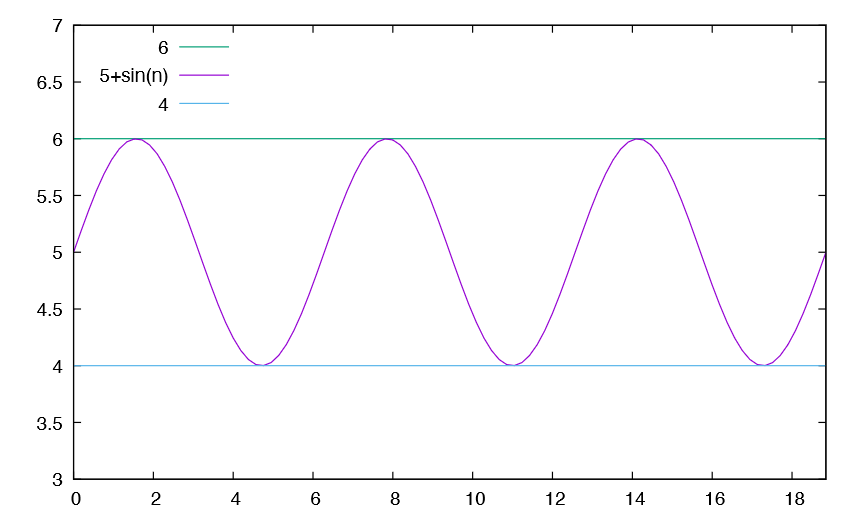
\includegraphics[scale=0.5]{02/graficoFsin.png}
    \subsection{Proprietà delle notazioni}
        \subsubsection{Dualità}
            $ f(n) = O(g(n)) \Leftrightarrow g(n) = \Omega(f(n)) $
            \begin{proof}
                $$
                    \begin{aligned}
                        f(n) = O(g(n)) \Leftrightarrow & f(n) \leq cg(n), \forall n\geq m \\
                        \Leftrightarrow & g(n) \geq \frac1cf(n), \forall n\geq m \\
                        \Leftrightarrow & g(n) \geq c'f(n), \forall n\geq m, c'=\frac1c \\
                        \Leftrightarrow & g(n) = \Omega(f(n))
                    \end{aligned}
                $$
            \end{proof}
        \subsubsection{Eliminazione di costanti}
            $$
                \begin{aligned}
                    f(n) &= O(g(n)) \Leftrightarrow af(n)=O(g(n)), \forall a>0 \\
                    f(n) &= \Omega(g(n)) \Leftrightarrow af(n)=\Omega(g(n)), \forall a>0 \\
                \end{aligned}
            $$
            \begin{proof}                
                $$
                    \begin{aligned}
                        f(n)=O(g(n)) \Leftrightarrow & f(n)\leq cg(n), \forall n\geq m \\
                        \Leftrightarrow & af(n)\leq acg(n), \forall n\geq m,\forall a>0 \\
                        \Leftrightarrow & af(n)\leq c'g(n), \forall n\geq m,c'=ac>0 \\
                        \Leftrightarrow & af(n)=O(g(n)), \forall a>0
                    \end{aligned}
                $$
            \end{proof}
        \subsubsection{Sommatoria (sequenza di algoritmi)}
            $$
                \begin{aligned}
                    f_1(n) = O(g_1(n)), f_2(n) = O(g_2(n)) \Rightarrow f_1(n) + f_2(n) = O(\max(g_1(n),g_2(n)))\\
                    f_1(n) = \Omega(g_1(n)), f_2(n) = \Omega(g_2(n)) \Rightarrow f_1(n) + f_2(n) = \Omega(\max(g_1(n),g_2(n)))
                \end{aligned}
            $$
            \begin{proof}[Dimostrazione (Lato $ O $).]
                $$
                    \begin{aligned}
                        f_1(n) = O(g_1(n)) \land f_2(n) = O(g_2(n)) & \Rightarrow \\
                        f_1(n) \leq c_1g_1(n) \land f_2(n) \leq c_2g_2(n) & \Rightarrow \\
                        f_1(n) + f_2(n) \leq c_1g_1(n) + c_2g_2(n) & \Rightarrow \\
                        f_1(n) + f_2(n) \leq \max\{c_1,c_2\}(2\cdot \max(g_1(n),g_2(n))) & \Rightarrow \\
                        f_1(n) + f_2(n) = O(\max(g_1(n),g_2(n))) &
                    \end{aligned}
                $$
            \end{proof}
        \subsubsection{Prodotto (cicli annidati)}
            $$
                \begin{aligned}
                    f_1(n) = O(g_1(n)), f_2(n) = O(g_2(n)) \Rightarrow f_1(n) \cdot f_2(n) = O(g_1(n) \cdot g_2(n))\\
                    f_1(n) = \Omega(g_1(n)), f_2(n) = \Omega(g_2(n)) \Rightarrow f_1(n) \cdot f_2(n) = \Omega(g_1(n) \cdot g_2(n))
                \end{aligned}
            $$
            \begin{proof}
                $$
                    \begin{aligned}
                        f_1(n) = O(g_1(n)) \land f_2(n) = O(g_2(n)) & \Rightarrow \\
                        f_1(n) \leq c_1g_1(n) \land f_2(n) \leq c_2g_2(n) & \Rightarrow \\
                        f_1(n)\cdot f_2(n) \leq c_1c_2g_1(n)g_2(n) &
                    \end{aligned}
                $$
        \end{proof}
        \subsubsection{Simmetria}
            $$
                f(n) = \Theta(g(n)) \Leftrightarrow g(n) = \Theta(f(n))
            $$
            \begin{proof}
                Grazie alla proprietà della dualità, si ha che:
                $$
                    \begin{aligned}
                        f(n) = \Theta(g(n)) &\quad \Rightarrow \quad f(n) = O(g(n)) \Rightarrow g(n) = \Omega(f(n))\\
                        f(n) = \Theta(g(n)) &\quad \Rightarrow \quad f(n) = \Omega(g(n)) \Rightarrow g(n) = O(f(n))
                    \end{aligned}
                $$
            \end{proof}
        \subsubsection{Transitività}
            $$
                \begin{aligned}
                    f(n) = O(g(n)), g(n) = O(h(n)) \Rightarrow f(n) = O(h(n))
                \end{aligned}
            $$
            \begin{proof}
                $$
                    \begin{aligned}
                        f(n) = O(g(n)) \land g(n) = O(h(n)) & \Rightarrow \\
                        f(n) \leq c_1g(n) \land g(n) \leq c_2h(n) & \Rightarrow \\
                        f(n) \leq c_1c_2h(n) & \Rightarrow \\
                        f(n) = O(h(n)) &
                    \end{aligned}
                $$
            \end{proof}
    \subsection{Altre funzioni di costo}
        \subsubsection{Logaritmi v/s funzioni lineari}
            \paragraph{Proprietà dei Logaritmi}
                Vogliamo provare che $ \log(n) = O(n) $. Dimostriamo per induzione che
                $$
                    \exists c>0,\exists m\geq 0:\log n\leq cn,\forall n\geq m\qquad \text{definizione di }O
                $$
                \begin{proof}
                    \begin{basecase} ($ n=1 $):
                        $ \log 1 = 0 \leq \stackrel{c}0\cdot \stackrel{n}1 = 0 $
                    \end{basecase}
                    \textbf{Ipotesi induttiva}: sia $ \log k \leq ck, \forall k\leq n $.
                    \begin{inductivecase}
                        Dimostriamo la proprietà per $ n+1 $:
                        $$
                            \begin{aligned}
                                \log(n+1) \leq & \log(n+n) = \log 2n & \forall n\geq 1 \\
                                = & \log 2 + \log n \qquad & \log ab = \log a + \log b \\
                                = & 1 + \log n & \log 2 = 1 \\
                                \leq & 1 + cn & \text{per induzione} \\
                                \stackrel{?}{\leq} & c(n+1) & \text{Obbiettivo} \\
                                1+cn\leq c(n+1) \Leftrightarrow & c\geq 1
                            \end{aligned}
                        $$
                    \end{inductivecase}
                \end{proof}
        \subsection{Giocando con le espressioni}
            \paragraph{Es 1}
                È vero che $ \log_a n = \Theta(\log n) $?

                Si: $ \log_a n = (\log_a 2) \cdot (\log_2 n) = \Theta(\log n) $
            
            \paragraph{Es 2}
                È vero che $ \log n^a = \Theta(\log n) $, per $ a>0 $?

                Si: $ \log n^a = a\log n = \Theta(\log n) $
            
            \paragraph{Es 3}
                È vero che $ 2^{n+1} = \Theta(2^n) $?

                Si: $ 2^{n+1} = 2\cdot 2^n = \Theta(2^n) $
            \paragraph{Es 4}    
                È vero che $ 2^{n} = \Theta(3^n) $?

                Ovviamente $ 2^{n} = O(3^n) $

                Ma: $ 3^{n} = \left(\frac32\cdot 2\right)^n=\left(\frac32\right)^n\cdot 2^n: $ Quindi non esiste $ c > 0 $ tale per cui $ \left(\frac32\right)^n\cdot 2^n\leq c2^n $, quindi $ 2^n \neq O(3^n) $
    \subsection{Classificazione delle funzioni}
        È possibile definire un ordinamento delle principali classi estendendo le relazioni che abbiamo dimostrato:
        
        Per ogni $r<s,h<k,a<b$:
        $$
            o(1) \subset O(\log^r n) \subset O(\log^s n) \subset O(n^h) \subset O(n^h \log^r n ) \subset O(n^h \log^s n) \subset O(n^k) \subset O(a^n) \subset O(b^n)
        $$
\section{Ricorrenze}
    \subsection{Introduzione}
        \paragraph{Equazioni di ricorrenza} Quando si calcola la complessità di un algoritmo ricorsivo, questa viene espressa tramite un'\textbf{equazione di ricorrenza}, ovvero una formula definita in maniera ricorsiva.
            \subparagraph{MergeSort}
                $$
                    T(n) = \begin{cases}
                        1 & \text{se } n=1 \\
                        2T\left(\frac{n}{2}\right) + n & \text{se } n>1
                    \end{cases}
                $$
        \paragraph{Forma Chiusa} L'obbiettivo è quello di ottenere, quando possibile, una \textbf{formula chiusa} che rappresenti la classe di complessità della funzione.
            \subparagraph{MergeSort}
                $$ 
                    T(n) = \begin{cases}
                        T(\lfloor n/2 \rfloor) + T(\lceil n/2 \rceil) + \Theta(n) & n > 1 \\
                        \Theta(1) & n \leq 1
                    \end{cases} \Longrightarrow T(n) = \Theta(n\log n)
                $$
    \subsection{Metodo dell'albero di ricorsione, o per livelli}
        \paragraph{Introduzione} "Srotoliamo" la ricorrenza in un albero i costi ai vari livelli della ricorsione.
        \subsubsection{Esempio 1}
            $$
                T(n)=\begin{cases}
                    T(n/2) + b & n>1 \\
                    c & n\leq 1
                \end{cases}
            $$
            È possibile risolvere questa ricorrenza nel modo seguente:
            $$
                \begin{aligned}
                    T(n) = & b + T(n/2) \\
                    = & b + b + T(n/4) \\
                    = & b + b + b + T(n/8) \\
                    = & \ldots \\
                    = & \underbrace{b+b+\ldots+b}_{\log n} + T(1) \\
                \end{aligned}
            $$
            Assumiamo per semplicità che $ n=2^k $. $ T(n) = b\log n + c = \Theta(\log n) $
        \subsubsection{Esempio 2}
            $$
                T(n)=\begin{cases}
                    4T(n/2) + n & n>1 \\
                    1 & n\leq 1
                \end{cases}
            $$
            È possibile risolvere questa ricorrenza nel modo seguente:
            $$
                \begin{aligned}
                    T(n)=&\cancel{n\sum_{j=0}^{\log(n-1)} 2^j} &\underbrace{+4^{\log n}}_{\text{somma degli }T(1)}\\
                    \Rightarrow &\underbrace{n\cdot \frac{\overbrace{2^{\log n }}^{n\text{ per prop. log.}}-1}{2-1}}_{\stackrel{\text{usando: }}{\forall x\neq 1:\sum_{j=0}^kx^j=\frac{x^{k+1}-1}{x-1}}}&+4^{\log n}\\
                    =& n(n-1)&+4^{\log n}\\
                    =& n^2-n&\overbrace{+n^2}^{\text{cambiamento di base}}\\
                    =& 2n^2-n = \Theta(n^2)
                \end{aligned}
            $$
        \subsubsection{Esempio 3}
        $$
            T(n)=\begin{cases} 4T(n/2) + n^3 & n>1 \\ 1 & n\leq 1 \end{cases}
        $$
        Da questa equazione notiamo che il primo livello ha costo $ n^3 $, il secondo $ 4\left(\frac{n}{2}\right)^3 $ il terzo $ 4^2\left(\frac{n}{2^2}\right)^3 $ e così via. Quindi possiamo scrivere la sommatoria:
        $$
            \begin{aligned}
                T(n)=& n^3 + 4\left(\frac{n}{2}\right)^3 + \ldots + 4^{\log n-1}\left(\frac{n}{2^{\log n-1}}\right)^3 &+ 4^{\log n} \\
                =& \sum_{i=0}^{\log n-1}4^i\left(\frac{n}{2^i}\right)^3 & + 4^{\log n} \\
                =& n^3\sum_{i=0}^{\log n-1}\left(\frac{2^{2i}}{2^{3i}}\right) & + 4^{\log n} \\
                =& n^3\sum_{i=0}^{\log n-1}\left(2^{2i-3i}\right) & + 4^{\log n} \\
                =& n^3\sum_{i=0}^{\log n-1}\left(2^{-1\cdot i}\right) & + 4^{\log n} \\
                =& n^3\sum_{i=0}^{\log n-1}\left(\frac{1}{2}\right)^i & \overbrace{+n^2}^{\text{cambiamento di base}} \\
                \leq & n^3\sum_{i=0}^{\infty}\left(\frac{1}{2}\right)^i & +n^2 \\
                =& n^3\cdot \overbrace{\frac{1}{1-\frac{1}{2}}}^{\text{usando: }\forall x,|x|\leq 1:\sum_{i=0}^{\infty}x^i=\frac{1}{1-x}} & +n^2 \\
                =& 2n^3 + n^2
            \end{aligned}
        $$
        \footnote{In quanto la sommatoria tende a crescere allora abbiamo potuto sostituire $ \log n $ con $ \infty $ e modificare il segno di uguaglianza con quello di $ \leq $ in quanto la sommatoria verso l'infinito converge è più grande di quella finita}\newline
        Abbiamo dunque dimostrato che $ T(n) \leq 2n^3 + n^2 = O(n^3) $ però non possiamo, tramite la dimostrazione precedente, dire che $ T(n) = \Theta(n^3) $ in quanto siamo passati ad una disequazione. In questo particolare caso d'altra parte possiamo notare che $ T(n) \geq n^3 $ il che ci porta ad affermare che $ T(n) = \Omega(n^3) $ e quindi $ T(n) = \Theta(n^3) $. 
    \subsection{Metodo di sostituzione}
        \paragraph{Introduzione} È il metodo in cui si cerca di \textbf{indovinare} (\textbf{guess}) la soluzione e si prova a dimostrarla per \textbf{induzione}.
        \subsubsection{Primo esempio}
            $$ T(n) = \begin{cases} T(\lfloor n/2 \rfloor) + n & n>1 \\ 1 & n\leq 1 \end{cases} $$
            Notiamo come il costo dei vali livelli sia $ n + n/2 + n/4 + \ldots $. Dunque possiamo ipotizzare di poter scrivere:
            $$
                \begin{aligned}
                    T(n)=& n \cdot \sum_{i=0}^{\log n}\left(\frac{1}{2}\right)^i\\
                    \leq & n \cdot \sum_{i=0}^{\infty}\left(\frac{1}{2}\right)^i\\
                    = & n \cdot \underbrace{\frac{1}{1-\frac{1}{2}}}_{\text{usando }\forall x,|x| < 1: \sum_{i=0}^{\infty}x^i=\frac{1}{1-x}}\\
                    = & 2n
                \end{aligned}
            $$
            \footnote{Abbiamo potuto usare il $ \leq $ in quanto la sommatoria in questione all'infinito è sempre maggiore di quella finita e ci stiamo calcolando il costo massimo}
            \paragraph{Limite superiore}
                Tentiamo quindi ora di dire che $ T(n) = O(n) $:
                \subparagraph{Caso Base} $ T(1) = 1 \stackrel{?}{\leq} 1 \cdot c \Leftrightarrow \forall c\geq 1 $
                \subparagraph{Passo Induttivo} Dimostriamo la disequazione per $T(n)$
                $$
                    \begin{aligned}
                        T(n) = & T(\lfloor n/2 \rfloor) + n \\
                        \leq & \overbrace{c\lfloor n/2 \rfloor}^{\text{ipotizzato} O(n)} + n \\
                        \leq & c\cdot\overbrace{n/2}^{\text{intero inferiore}} + n \\
                        = & n(c/2 + 1) \\
                        \stackrel{?}{\leq} & cn \\
                        \Leftrightarrow & c/2 + 1 \leq c \Leftrightarrow c\geq 2
                    \end{aligned}
                $$
                
                Dunque abbiamo provato che: $ T(n) \leq cn $, nel caso base $ c\geq 1 $ e nel passo induttivo $ c\geq 2 $. In quanto deve valere per entrambi i casi allora il primo valore utile di $ c $ è $2$, avendo provato che per $ n=1 $ la disequazione vale e che per tutti i successivi valori di $ n $ la disequazione vale allora possiamo dire che $ T(n) = O(n) $.
            \paragraph{Limite Inferiore}
                Tentiamo di dimostrare che $ T(n) = \Omega(n) $:
                \subparagraph{Caso Base} Dimostriamo che $ T(1) = 1 \stackrel{?}{\geq} 1\cdot d \Leftrightarrow \forall d\leq 1 $
                \newpage % Per evitare che il passo induttivo vada a capo
                \subparagraph{Passo Induttivo} Dimostriamo la disequazione per $ T(n) $:
                $$
                    \begin{aligned}
                        T(n) =& T(\lfloor n/2 \rfloor) + n \\
                        \geq & \overbrace{d\lfloor n/2 \rfloor}^{\text{per ipo. induttiva sostituzione}} + n \\
                        \geq & d\cdot\overbrace{\frac{n}2-1}^{\text{intero inferiore}} + n \\
                        = & \left(\frac{d}2-\frac1n+1\right)n \stackrel{?}{\geq} dn \\
                        \Leftrightarrow & \frac{d}2-\frac1n+1 \geq d \\ 
                        \Leftrightarrow & d\leq 2 - \frac2n
                    \end{aligned}
                $$

                Abbiamo quindi dimostrato che $ T(n) \geq dn $, nel caso base $ d\leq 1 $ e nel passo induttivo $ d\leq 2 - \frac2n $. In quanto deve valere per entrambi i casi allora il primo valore utile di $ d $ è $1$, avendo provato che per $ n=1 $ la disequazione vale e che per tutti i successivi valori di $ n $ la disequazione vale allora possiamo dire che $ T(n) = \Omega(n) $.
                
            \paragraph{Conclusione} Avendo provato che $ T(n) = O(n) $ e $ T(n) = \Omega(n) $ e ricordando che se $ T(n) = O(n) \land T(n) = \Omega(n) \Leftrightarrow T(n) = \Theta(n) $ concludendo che la funzione di costo di $ T(n) $ cresce in maniera lineare.
        \subsubsection{Terzo esempio - Difficoltà matematiche}
            $$
                T(n)=\begin{cases} T\left(\left\lfloor\frac{n}2\right\rfloor\right) + T\left(\left\lceil\frac{n}2\right\rceil\right) + 1 & n>1 \\ 1 & n\leq 1 \end{cases}
            $$
            \paragraph{Limite Superiore}
                Dalla seguente si può notare come il costo di ogni livello sia $ 1 $ e che il numero di livelli sia $ \log n $. Inoltre la ricorsione viene eseguita su due rami, quindi possiamo scrivere la seguente sommatoria:
                $$
                    \begin{aligned}
                        T(n)=&\sum_{i=0}^{\log n}2^i\\
                        =&1+2+4+\ldots+\frac{n}4+\frac{n}2+n \\
                        =&O(n)
                    \end{aligned}
                $$
                Proviamo ora a dimostrare che $ T(n) = O(n) $:
                \subparagraph{Passo Induttivo} Ipotizzando che $ \forall k<n:T(k)\leq ck $, dimostriamo che $ T(n)\leq cn $:
                    $$
                        \begin{aligned}
                            T(n)=&T\left(\left\lfloor\frac{n}2\right\rfloor\right) + T\left(\left\lceil\frac{n}2\right\rceil\right) + 1 \\
                            \leq & c\left\lfloor\frac{n}2\right\rfloor + c\left\lceil\frac{n}2\right\rceil + 1 \\
                            \leq & cn+1 \\
                            \stackrel{?}{\geq} & cn \Rightarrow 1\leq 0 & \text{ impossibile}
                        \end{aligned}
                    $$
                    Sebbene la dimostrazione sia fallita ma l'intuizione ci dice che $ T(n) = O(n) $

                Proviamo dunque a dimostrarlo per un \textbf{ordine inferiore}: $ cn+1\leq cn $
                \subparagraph{Passo Induttivo} Ipotizzando che $ \exists b>0,\forall k<n:T(k)\leq ck-b $ allora dimostriamo la disequazione per $T(n)$:
                    $$
                        \begin{aligned}
                            T(n)=&T\left(\left\lfloor\frac{n}2\right\rfloor\right) + T\left(\left\lceil\frac{n}2\right\rceil\right) + 1 \\
                            \leq & c\left\lfloor\frac{n}2\right\rfloor - b + c\left\lceil\frac{n}2\right\rceil - b + 1 \\
                            =& cn - 2b + 1 \\
                            \stackrel{?}{\leq} & cn - b \\
                            \Rightarrow & \cancel{cn} - 2b + 1 \leq \cancel{cn} - b \Rightarrow b\geq 1
                        \end{aligned}
                    $$
                    Dimostriamo il passo base per $ b=1 $: $ T(1) = 1 \stackrel{?}{\leq} 1\cdot c - b\Leftrightarrow \forall c\geq b+1 $
            \paragraph{Limite Inferiore} 
                Proviamo ora a dimostrare che $ T(n) = \Omega(n) $:
                \subparagraph{Passo Induttivo} Ipotizzando che $ \forall k<n:T(k)\geq dk $, dimostriamo che $ T(n)\geq dn $:
                    $$
                        \begin{aligned}
                            T(n)=&T\left(\left\lfloor\frac{n}2\right\rfloor\right) + T\left(\left\lceil\frac{n}2\right\rceil\right) + 1 \\
                            \geq & d\left\lfloor\frac{n}2\right\rfloor + d\left\lceil\frac{n}2\right\rceil + 1 \\
                            = & dn + 1 \\
                            \stackrel{?}{\geq} & dn \Rightarrow 1\geq 0 
                        \end{aligned}
                    $$ Il che è vero $ \forall d $ in quanto $ d $ è positivo per ipotesi.
                \subparagraph{Caso base} Dimostriamo la disequazione per $ T(1) $:
                    $$
                        T(1) = 1 \geq 1\cdot d \Leftrightarrow d\leq 1
                    $$Dunque abbiamo provato che $ T(n) = \Omega(n) $

                Avendo dimostrato in precedenza che $ T(n) = O(n) $ e $ T(n) = \Omega(n) $ possiamo concludere che $ T(n) = \Theta(n) $ e quindi la funzione di costo cresce linearmente.
    \subsection{Metodo dell'esperto, o delle ricorrenze comuni}
        \paragraph{Riccorenze comuni} Esiste un'ampia classe di ricorrenze che si risolvono facilmente facendo ricorso a qualche teorema, ogni teorema è applicabile ad una particolare classe di ricorrenze.
        \subsubsection{Ricorrenze lineari con partizione bilanciata}
            \begin{theorem}
                Siano $ a,b $ costanti intere tali che $ a \geq 1 $ e $ b \geq 2 $, e esistano $c,\beta$ costanti reali tali che $ c > 0 $ e $ \beta \geq 0 $. Sia $ T(n) $ data dalla seguente relazione di ricorrenza:
                \begin{align}
                    T(n)=\begin{cases}
                        aT(n/b) + cn^\beta & n>1 \\
                        1 & n\leq 1
                    \end{cases}
                \end{align}
                Posto: $\alpha = \frac{\log a}{\log b}= \log_b a$ allora:
                \begin{align}
                    T(n)=\begin{cases}
                        \Theta(n^\alpha) & \alpha > \beta \\
                        \Theta(n^\alpha\log n) & \alpha = \beta \\
                        \Theta(n^\beta) & \alpha < \beta
                    \end{cases}
                \end{align}
            \end{theorem}
            \paragraph{Assunzioni} Assumiamo che $ n $ sia una potenza intera di $ b $, ovvero $ n=b^k, k=\log_bn $.
                \subparagraph{Influisce sul risultato?}
                    \begin{itemize}
                        \item Supponendo che l'input abbia dimensione $b^{k}+1$
                        \item Estendiamo l'input fino alla dimensione $b^{k+1}$ (\textbf{padding})
                        \item L'input è stato esteso di un fattore $b$
                        \item Il che non cambia la complessità computazionale
                    \end{itemize}
            \paragraph{Dimostrazione caso 1}
            \paragraph{Dimostrazione caso 2} $\alpha = \beta $
            \begin{proof}
                Ne segue che: $q=b^{\alpha-\beta}=1$ e dunque la funzione $T(n)$:
                \begin{align}
                    T(n)=&dn^\alpha+cb^{k\beta}\sum_{i=0}^{k-1}q^i\\
                    =&n^\alpha d+cn^\beta k \qquad & q^i=1^i=1\\
                    =&n^\alpha d+cn^\alpha k & \alpha = \beta\\
                    =&n^\alpha(d+ck)\\
                    =&n^\alpha\left[d+c\frac{\log n}{\log b}\right] & k=\log_b n
                \end{align}
            \end{proof}
            e come conseguenza $T(n)=\Theta(n^\alpha\log n)$
\end{document}